\documentclass[conference]{IEEEtran}
\IEEEoverridecommandlockouts
\usepackage{cite,amsmath,graphicx,booktabs,url,xcolor}
\usepackage[hidelinks]{hyperref}
\usepackage{pgfplots}
\pgfplotsset{compat=1.17}

\begin{document}

\title{Live Allocation-Aware Resource Advising on Chameleon:\\
Corpus Triage, Blazar Integration, and Targeted Availability Fetch}

\author{\IEEEauthorblockN{Vivek Rai}
\IEEEauthorblockA{Chameleon Fellowship\\
chi-edge-advisor / benchmark\_v4}}

\maketitle

\begin{abstract}
We report three connected pieces of work on the Chameleon resource advisor.
First, a deterministic ingestion pipeline over the 205-artifact Trovi catalog,
which establishes that only 95 artifacts contain Chameleon provisioning code at
all and only 90 are usable for resource recommendation. Second, replacement of
the advisor's non-functional \texttt{python-chi} availability path with a direct
Blazar REST client covering all seven Chameleon sites, adding reservation time
windows and a previously invisible third node state. Third, a resource catalog
mapping node types to sites, enabling targeted fetches that cut availability
latency by up to $10.8\times$. We also record the architectural decision to
abandon the hierarchical artifact router in favour of a flat, tag-indexed JSON
store, which measurement shows is not merely simpler but more accurate.
\end{abstract}

\begin{IEEEkeywords}
testbed provisioning, resource allocation, Blazar, retrieval, reproducibility
\end{IEEEkeywords}

\section{Frozen-Measurement Baseline}

All downstream work is diffed against a pinned baseline so corpus expansion
cannot silently perturb the benchmark. Capturing it exposed that the committed
baseline was already stale: it recorded 406 empty / 150 scored cells, while the
\texttt{runs/} files committed in the \emph{same} commit rescore to 314 / 242.
There was, in effect, no valid baseline before this work.

\begin{table}[h]
\caption{Pinned parity artifact (556 cells, 242 non-empty)}
\label{tab:parity}
\centering\footnotesize
\begin{tabular}{@{}ll@{}}
\toprule
Artifact & sha256 (truncated) \\
\midrule
\texttt{run\_scores.csv}      & \texttt{252e42bf\ldots1387525} \\
\texttt{gate\_report.json}    & \texttt{d51facdb\ldots71f3da6e} \\
content manifest (63 files)   & \texttt{e26c9537\ldots cac9505a} \\
\bottomrule
\end{tabular}
\end{table}

The gold gate passes 50/50 and the pin re-verifies byte-identically. Physical
separation does the enforcing: nothing the pipeline produces is written to
\texttt{benchmark\_v4/grounding/}, because \texttt{run\_bench.py:90} and
\texttt{tier\_assign.py:33} glob those paths and the frozen provenance hash
depends on them.

\section{Corpus Triage: the Real \emph{N}}

The 205 catalog artifacts were fetched (180 cloned, 20 sparse-checkout above a
200\,MB cap, 7 unfetchable) and classified by AST-based detection of the
measured \texttt{python-chi} call surface.

\begin{table}[h]
\caption{Triage outcome over 205 Trovi artifacts}
\label{tab:triage}
\centering\footnotesize
\begin{tabular}{@{}lrl@{}}
\toprule
Class & $n$ & Consequence \\
\midrule
no-chameleon-code & 108 & unusable: no provisioning grammar \\
instructional     & 49  & tutorial-shaped grounding \\
evidence          & 46  & research-shaped grounding \\
excluded          & 2   & policy (v1 overlap, explicit) \\
\midrule
\textbf{usable}   & \textbf{95} & \textbf{real \emph{N}, not 205} \\
\bottomrule
\end{tabular}
\end{table}

\textbf{This is the headline planning number.} 53\,\% of the catalog carries no
Chameleon provisioning code, typically because the GitHub link points at
upstream paper code while the provisioning lives in the Trovi body. Ranking the
95 by how much of a \emph{groundable} resource recommendation can be extracted
narrows it further: 39 tier-A and 51 tier-B, so \textbf{90 artifacts} are worth
ingesting. Any plan sized on 205 is roughly $2\times$ over.

A secondary finding cuts the other way. The new corpus contains \textbf{52
artifacts using \texttt{add\_node\_reservation}}, where the existing workspace
had the bare-metal grammar zero times outside \texttt{forbidden\_calls} trap
lists. The corpus supplies exactly the positive examples the emitter lacks.

Detection was cross-checked against an independent regex sweep over all 102
inspectable negatives: \emph{one} true false negative, caused by a 9.4\,MB
notebook skipped by a byte cap. Notebook size is driven by embedded output
images rather than code, so the cap now applies to extracted source.

\section{Architecture: Tree $\rightarrow$ Tag-Indexed Store}

The advisor was originally designed around a hierarchical router:
site $\rightarrow$ use-case $\rightarrow$ artifact (\texttt{RouterTree}). We
abandoned it for a flat store with JSON tag records. This was not simplification
for its own sake; the hierarchy measurably retrieves worse.

\begin{table}[h]
\caption{Router ablation A7, artifact hit rate (45 covered items)}
\label{tab:a7}
\centering\footnotesize
\begin{tabular}{@{}lcc@{}}
\toprule
Level & Tree & Flat + tags \\
\midrule
L0 site            & 100.0\,\% & n/a \\
L1 use-case @2     & 73.3\,\%  & n/a \\
L2 artifact @3     & 68.9\,\%  & \textbf{86.7\,\%} \\
chunk-level        & 68.9\,\%  & \textbf{86.7\,\%} \\
\bottomrule
\end{tabular}
\end{table}

The tree loses 17.8 points at the artifact level. The cause is structural: every
hard gate is a place to be irrecoverably wrong. A use-case misclassification at
L1 removes the correct artifact from consideration before L2 ever runs, and the
L1 gate is only 73.3\,\% accurate. Flat scoring lets a weak signal on one facet
be outvoted rather than becoming fatal.

The corpus is therefore stored as flat tagged records, not a hierarchy:
\texttt{catalog.jsonl}, \texttt{manifest.tsv} (18 columns), and
\texttt{resource\_catalog.json}. Two orthogonal tag vocabularies are emitted
rather than one taxonomy, because the advisor performs a \emph{mapping}: 23
workload tags on the query side (what the user wants) and 13 resource tags on
the answer side (what that implies about hardware). Resource tags derive only
from observed code, never prose, since that half is what the emitter renders.
TSV was chosen over JSON for the scan table on a measured 57 versus 238 tokens
per row, paid 200 times.

\section{Live State: Blazar, Not the Reference API}

The advisor's availability layer did not work. The public reference API is
\textbf{static-only} and exposes zero CHI@Edge inventory; its deeper endpoints
currently return 500/502. The \texttt{python-chi} backend failed at its own
site-discovery call and saw only one site. We replaced it with direct REST:
Keystone \texttt{/auth/tokens} $\rightarrow$ service catalog $\rightarrow$
Blazar $\rightarrow$ \texttt{\{resource\}} + \texttt{/allocations}.

Three findings shaped the design.

\textbf{(1) Blazar has no server-side filter.} Measured, not assumed:
\texttt{?node\_type=}, \texttt{?q=}, \texttt{?filter=} and \texttt{?query=} all
return HTTP 200 with \emph{all} 132 hosts. Narrowing is therefore possible only
by contacting fewer \emph{sites}.

\textbf{(2) Reservations do not name their hosts.} Reading \texttt{/leases}
alone finds nothing reserved and reports every host free, even at a site with an
active lease. The mapping lives on a separate \texttt{/allocations} endpoint.
This single correction moved the answer from ``587 free of 587'' to
Table~\ref{tab:fleet}.

\textbf{(3) There is a third state.} \texttt{reservable=false} is neither free
nor reserved. A node in maintenance is unbookable, and reporting it free is
precisely the failure that yields a spec that cannot be submitted.
\textbf{111 of 655 nodes} were in that state, previously counted as free.

\begin{table}[h]
\caption{Live Chameleon fleet, all seven sites}
\label{tab:fleet}
\centering\footnotesize
\begin{tabular}{@{}llrrrr@{}}
\toprule
Site & Resource & Free & Busy & Down & Total \\
\midrule
CHI@Edge  & devices  & 35  & 0   & 33  & 68  \\
CHI@NCAR  & os-hosts & 35  & 8   & 1   & 44  \\
CHI@NRP   & os-hosts & 0   & 0   & 4   & 4   \\
CHI@NU    & os-hosts & 6   & 0   & 2   & 8   \\
CHI@TACC  & os-hosts & 112 & 181 & 21  & 314 \\
CHI@UC    & os-hosts & 18  & 93  & 21  & 132 \\
KVM@TACC  & os-hosts & 2   & 54  & 29  & 85  \\
\midrule
\textbf{Total} & & \textbf{208} & \textbf{336} & \textbf{111} & \textbf{655} \\
\bottomrule
\end{tabular}
\end{table}

CHI@Edge required separate discovery: it answers \texttt{/devices}, not
\texttt{/os-hosts}, and its machine type lives in \texttt{machine\_name}
(\texttt{device\_type} is uniformly \texttt{"container"}). Every GPU class of
interest (A100, V100, H100) was fully reserved at capture time, leaving only
older silicon free. That contention is exactly what the advisor exists to
reason about. Per-node reservation windows are also now recorded, so the
advisor can answer ``free for how long'' and ``if not, when'' rather than only
``free now''.

\section{Targeted Fetch}

Because filtering must happen at site granularity, we persist a node-type
$\rightarrow$ site catalog refreshed by a full sweep. The distribution makes
this worthwhile: of 41 distinct types, \textbf{37 live on exactly one site}
(2 on two, 2 on three), a mean of 1.15 sites per type.

\begin{table}[h]
\caption{Availability fetch latency, measured}
\label{tab:speed}
\centering\footnotesize
\begin{tabular}{@{}lrrrr@{}}
\toprule
Request & Sites & Nodes & Time & Speedup \\
\midrule
Full sweep (baseline)      & 7 & 655 & 34.9\,s & $1.0\times$ \\
\texttt{compute\_skylake}  & 3 & 57  & 18.9\,s & $1.8\times$ \\
\texttt{gpu\_rtx\_6000}    & 1 & 37  & 7.5\,s  & $4.7\times$ \\
Pi camera workload         & 1 & 46  & \textbf{3.2\,s} & $\mathbf{10.8\times}$ \\
\bottomrule
\end{tabular}
\end{table}

\begin{figure}[h]
\centering
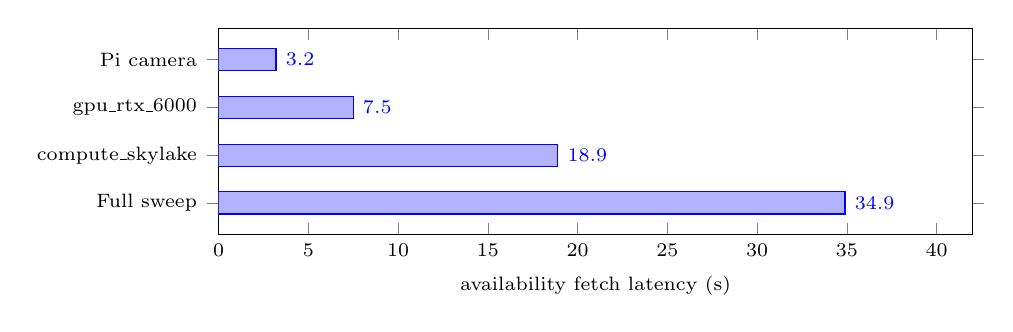
\begin{tikzpicture}
\begin{axis}[
  width=0.92\columnwidth, height=4.2cm,
  xbar, xmin=0, xmax=42,
  xlabel={availability fetch latency (s)},
  symbolic y coords={Pi camera,gpu\_rtx\_6000,compute\_skylake,Full sweep},
  ytick=data, y dir=reverse,
  nodes near coords, nodes near coords align={horizontal},
  every node near coord/.append style={font=\scriptsize},
  tick label style={font=\scriptsize}, label style={font=\scriptsize},
  bar width=8pt, enlarge y limits=0.22,
]
\addplot coordinates {(3.2,Pi camera) (7.5,gpu\_rtx\_6000)
                      (18.9,compute\_skylake) (34.9,Full sweep)};
\end{axis}
\end{tikzpicture}
\caption{Targeted fetch versus full sweep. The saving scales with how few sites
carry the requested type.}
\label{fig:speed}
\end{figure}

The pipeline was reordered to exploit this. Retrieval reads only the workload
string and the artifact registry, so it can run \emph{before} any network call
and tell the availability layer which hardware to ask about:
\[
\text{RETRIEVE} \rightarrow \text{READ} \rightarrow \text{REASON}
\rightarrow \text{VALIDATE} \rightarrow \text{EMIT}
\]
End to end, the pi-camera workload now contacts one site and sees 46 devices
instead of 655, and still validates \textsc{pass}.

Two guards prevent the optimisation from causing wrong answers, since pruning
incorrectly is worse than not pruning. An unrecognised type falls back to the
full sweep rather than pruning to an empty set. If the reasoner names a type
outside the candidate set, one targeted re-fetch runs (measured 3.5\,s) instead
of returning empty availability, which would fail
\texttt{device\_free\_in\_window} and silently turn a good recommendation into a
non-zero exit.

\section{Multi-Site Emission}

\texttt{Recommendation} now carries \texttt{site} and \texttt{api\_family},
copied from the catalog rather than inferred, and the emitter dispatches to
three genuinely distinct grammars.

\begin{table}[h]
\caption{Emitter dispatch, verified}
\label{tab:emit}
\centering\footnotesize
\begin{tabular}{@{}llll@{}}
\toprule
Family & Types & Reservation call & Boot \\
\midrule
edge      & 7  & \texttt{add\_device\_reservation} & \texttt{Container} \\
baremetal & 31 & \texttt{add\_node\_reservation}   & \texttt{Server} \\
kvm       & 3  & \texttt{add\_flavor\_reservation} & \texttt{Server} \\
\bottomrule
\end{tabular}
\end{table}

\textbf{Stated plainly:} the bare-metal template is written from the
\texttt{python-chi} API, not from anything observed locally, because
\texttt{add\_node\_reservation} and \texttt{create\_server} appear zero times as
real calls in this workspace. Both non-edge templates carry an
\textsc{unvalidated grammar} banner and are excluded from live dry-check. They
are also unreachable in practice today: all five registry artifacts are
\texttt{site="CHI@Edge"}, so routing never selects non-edge hardware. The
dispatch is ready; grounding it is the next task.

\section{Remaining Work}

\begin{enumerate}\itemsep2pt
\item \textbf{Ingest the 90 tier-A/B artifacts} into the registry. This is the
blocking item: multi-site emission is structurally complete but ungrounded, so a
GPU-training query still routes to a Raspberry Pi.
\item \textbf{Teach reservation from artifacts} --- what to reserve and how ---
grounding the bare-metal and KVM grammars against the 52 newly available
\texttt{add\_node\_reservation} examples.
\item \textbf{Schedule the catalog refresh.} A 168\,h TTL safety net exists but
nothing schedules the sweep, so it can stall a user call by $\sim$35\,s.
\item \textbf{Phase-1 adversarial audit} of the 10 selected artifacts, then the
25-artifact stratified phase 2. Seven strata have only one member.
\item \textbf{Recover \texttt{device\_profiles} for non-edge} types, and resolve
the 4 Trovi-hosted artifacts unreachable while the Trovi API returns 404.
\end{enumerate}

\section{Conclusion}

The corpus is half the size it appeared: 95 of 205 artifacts carry provisioning
code, and 90 are worth ingesting. The advisor now reads genuinely live state
across all seven sites, including a maintenance state covering 17\,\% of the
fleet that was previously reported as free. Targeted fetching makes that state
cheap enough to consult on every query, at up to $10.8\times$ less latency. The
architectural lesson worth carrying forward is the router ablation: the
hierarchical design was intuitive and measurably worse, because every hard gate
is a chance to be irrecoverably wrong.

Throughout, the frozen 556-cell measurement surface verified byte-identical and
the advisor test suite remained at 38/38.

\end{document}
